\chapter{测试与结果分析}

\section{实验环境与证据材料}
本文实验使用 IXI T1 脑部 MRI 数据作为主要数据来源。原始数据为 NIfTI 体数据，预处理后被转换为 PNG 二维切片，随后再打包为 StyleGAN2 训练数据集。根据训练配置文件，StyleGAN2 使用的数据集为 \texttt{mri128.zip}，最大训练切片数量为 60815 张，图像分辨率为 $128\times128$。

3DGS 实验使用连续 MRI 切片序列作为三维训练输入。训练集包含 180 张 $256\times256$ 切片，系统使用 300000 个初始点作为三维高斯优化起点。上述设置均可在项目训练目录中的相机参数、输入点云和训练日志中查到。

实验结论需要能够回到具体文件进行核对。本文使用真实项目产物作为证据材料，包括训练配置、日志文件、模型权重、生成切片、点云文件、3DGS checkpoint、渲染图像和指标统计结果。这些材料来自项目源码目录和结果目录，覆盖数据处理、二维生成、三维重建和平台测试等关键环节。

\begin{table}[H]
\centering
\caption{实验与测试证据材料}
\begin{tabular}{>{\raggedright\arraybackslash}p{4.1cm}>{\raggedright\arraybackslash}p{6.4cm}p{2.1cm}}
\toprule
证据材料 & 项目路径 & 状态 \\
\midrule
StyleGAN2 训练配置 & \thesispath{results/training_runs/00000-.../training_options.json} & 已确认 \\
StyleGAN2 训练日志 & \thesispath{results/training_runs/00000-.../log.txt} & 已确认 \\
可加载模型权重 & \thesispath{results/training_runs/network-snapshot-010000.pkl} & 已确认 \\
训练样本网格 & \thesispath{results/training_runs/00000-.../reals.png} & 已确认 \\
生成切片示例 & \thesispath{results/generated_slices/seed0042.png} 等 & 已确认 \\
初始点云文件 & \thesispath{results/3d_model_test/init_point_cloud.ply} & 已确认 \\
3DGS 训练日志 & \thesispath{results/3dgs_runs/mri_180slices_.../train.log} & 已确认 \\
3DGS 模型权重 & \thesispath{results/3dgs_runs/mri_180slices_.../chkpnt30000.pth} & 已确认 \\
3DGS 输出点云 & \thesispath{results/3dgs_runs/mri_180slices_.../point_cloud/iteration_30000/point_cloud.ply} & 已确认 \\
3DGS 渲染结果 & \thesispath{results/3dgs_runs/mri_180slices_.../train/ours_30000/renders} & 已确认 \\
\bottomrule
\end{tabular}
\end{table}

\section{StyleGAN2 训练配置与结果}
StyleGAN2 训练采用单 GPU 配置。Batch size 设置为 4，配置训练量为 25000 kimg。生成器和判别器均使用 Adam 优化器，学习率为 0.0025。潜变量维度和中间潜变量维度均为 512。训练过程中启用 ADA 数据增强，目标值为 0.6。训练输出目录保存训练配置、训练日志、真实样本网格和模型权重快照。

\begin{table}[H]
\centering
\caption{StyleGAN2 训练主要参数}
\begin{tabular}{p{4cm}p{8cm}}
\toprule
参数项 & 参数值 \\
\midrule
训练数据 & \texttt{mri128.zip} \\
图像分辨率 & $128\times128$ \\
训练切片数量 & 60815 \\
GPU 数量 & 1 \\
Batch Size & 4 \\
配置训练量 & 25000 kimg \\
模型快照 & \texttt{network-snapshot-010000.pkl} \\
优化器 & Adam \\
学习率 & 0.0025 \\
ADA 目标值 & 0.6 \\
\bottomrule
\end{tabular}
\end{table}

训练样本网格如图 \ref{fig:stylegan2-reals} 所示。该图来自训练输出目录中的 \texttt{reals.png}，可用于确认训练集是否被正确读取。样本网格中的输入样本为单通道脑部 MRI 切片，图中可以看到脑部轮廓和灰度层次。从实验观察看，预处理后的切片灰度范围较稳定，能够作为二维生成模型的训练输入。

\begin{figure}[H]
\centering
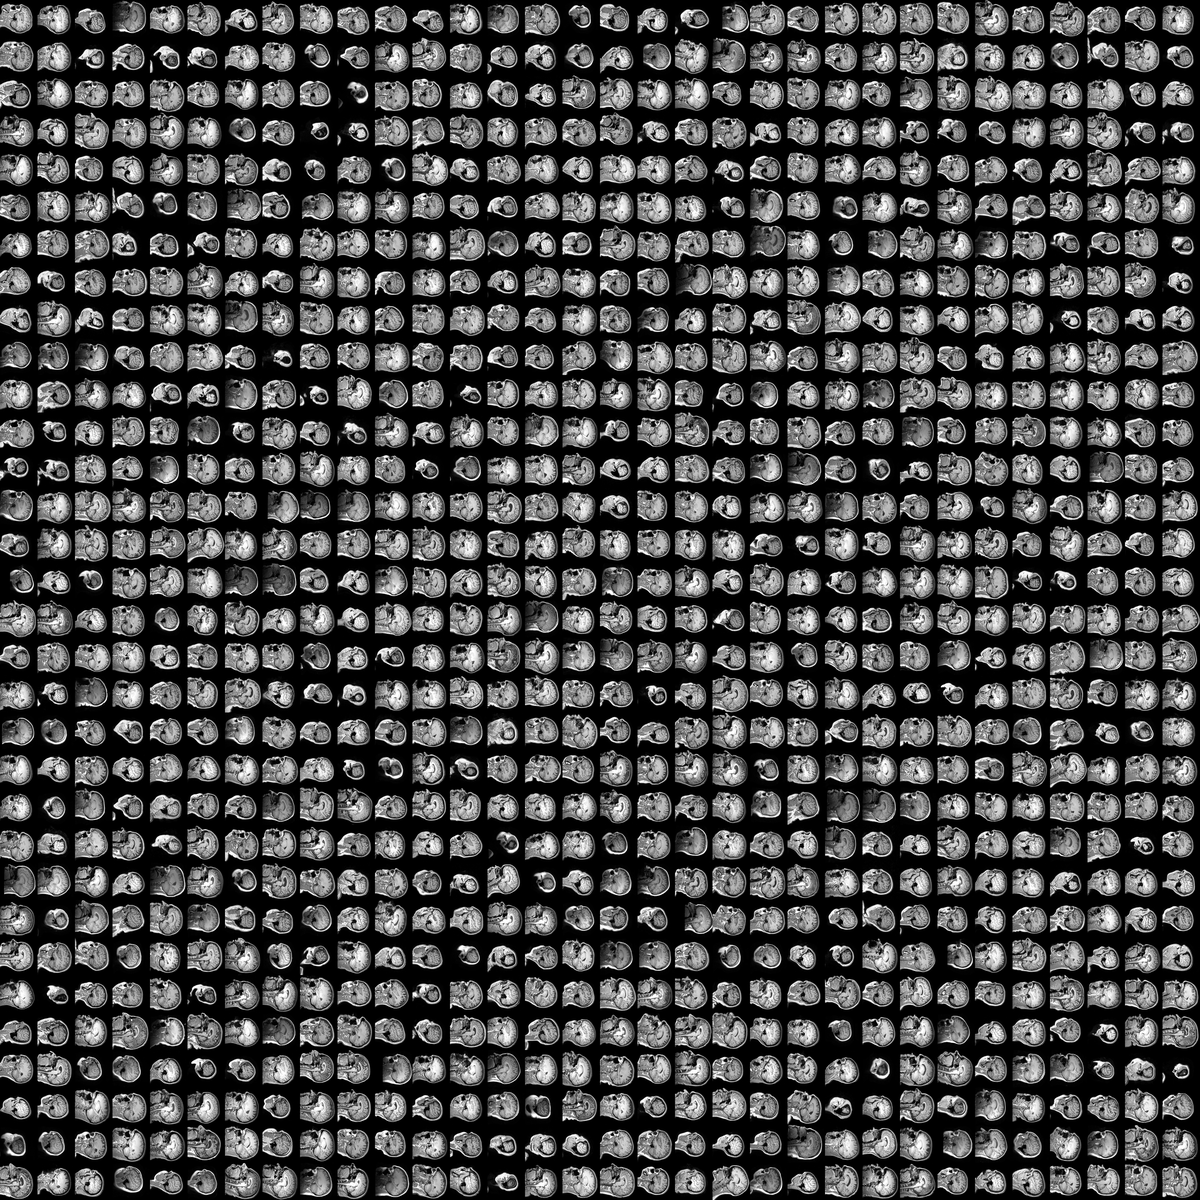
\includegraphics[width=0.82\textwidth]{figures/stylegan2_reals_preview.png}
\caption{StyleGAN2 训练集中真实 MRI 切片样本网格}
\label{fig:stylegan2-reals}
\end{figure}

训练完成后，项目得到可加载的模型快照 \texttt{network-snapshot-010000.pkl}。平台能够读取该权重并生成 MRI 切片，说明权重加载、潜变量采样、生成器推理、图像张量转换和 PNG 保存等环节已经连通。本文评价 StyleGAN2 结果时，重点不放在临床诊断性能上，而是关注生成链路可用性、输出可复现性和对三维输入的支撑能力。

\section{二维切片生成结果分析}
平台生成的示例切片如图 \ref{fig:generated-slices} 所示。该图来自生成切片结果目录，图像由训练完成的 StyleGAN2 权重生成。不同随机种子对应不同潜变量输入，系统由此得到不同灰度分布和结构形态的 MRI 切片示例。图中结果呈现出脑部 MRI 切片的基本轮廓和灰度结构，说明平台推理模块能够正确调用训练权重。

\begin{figure}[H]
\centering
\begin{subfigure}{0.32\textwidth}
\centering
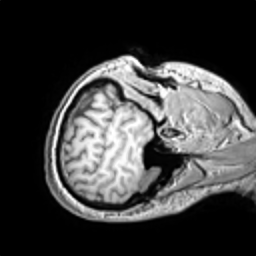
\includegraphics[width=\textwidth]{figures/generated_seed0123.png}
\caption{随机种子 123}
\end{subfigure}
\hspace{0.08\textwidth}
\begin{subfigure}{0.32\textwidth}
\centering
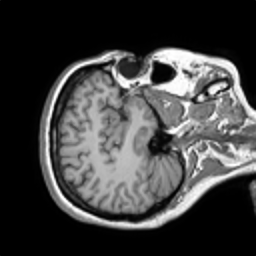
\includegraphics[width=\textwidth]{figures/generated_seed0042.png}
\caption{随机种子 42}
\end{subfigure}
\caption{StyleGAN2 生成的 MRI 切片示例}
\label{fig:generated-slices}
\end{figure}

二维切片生成链路已经形成闭环。用户在平台中指定模型权重、生成数量、截断参数和随机种子后，系统完成潜变量采样、生成器前向推理、灰度图像转换和结果保存。截断参数 \texttt{truncation\_psi} 用于调节生成结果的稳定性和多样性，随机种子则保证同一参数组合下结果可复现。该功能既可产生论文展示图，也可作为连续切片序列和点云初始化的输入。

\section{平台功能测试}
平台功能测试关注主要流程是否按预期运行。测试内容包括 FastAPI 后端接口、React 前端页面、数据预处理、模型训练入口、切片生成、连续序列生成、点云初始化、3DGS 结果展示和 AI 助手。测试结果显示，FastAPI 后端服务可以正常启动，React 前端可以访问平台页面；生成模块能够调用训练完成的权重输出 PNG 切片；点云初始化模块能够从切片目录生成 PLY 文件；3DGS 训练结果也能够以日志、渲染图像和点云文件形式归档。

\begin{table}[H]
\centering
\caption{平台主要功能测试结果}
\begin{tabular}{>{\raggedright\arraybackslash}p{3cm}>{\raggedright\arraybackslash}p{5.2cm}>{\raggedright\arraybackslash}p{4.8cm}}
\toprule
测试模块 & 测试内容 & 测试结果 \\
\midrule
数据预处理 & NIfTI 读取、轴向切片、归一化、缩放和 PNG 保存 & 已实现，可按数据目录批量处理 \\
模型训练 & 自动识别训练数据并启动 StyleGAN2 训练 & 已实现，训练结果已存在 \\
切片生成 & 加载 \texttt{.pkl} 权重并生成 PNG 图像 & 已通过，已有生成样例 \\
连续序列 & 潜空间插值得到连续切片序列 & 已实现，可用于三维展示 \\
点云初始化 & 将切片序列转换为 PLY 点云 & 已通过，已有 PLY 结果 \\
3DGS 重建 & 组织切片、点云、相机参数并完成训练输出 & 已通过，已有 checkpoint、点云和渲染结果 \\
FastAPI 后端 & 提供概览、生成、资产、任务、分析、报告和 AI 助手接口 & 已实现，可由 React 前端调用 \\
React 前端 & 提供仪表盘、生成、查看器、报告、可信性评估、任务、3D 和教学页面 & 已实现，可通过 Vite 本地服务访问 \\
AI 助手 & 参数说明和平台问答 & 已实现，包含本地解释逻辑和可选搜索接口 \\
\bottomrule
\end{tabular}
\end{table}

测试过程表明，平台已经具备毕业设计所需的演示能力。用户可以通过 React 前端完成从结果查看到二维生成，再到医学影像分析、可信性评估、三维表达和 3DGS 结果展示的主要流程。FastAPI 后端负责接口封装、任务状态和结果资产输出。平台首页、生成工作台、影像查看器、任务中心、点云展示页和异常提示共同构成系统展示材料。

\section{点云初始化结果分析}
点云初始化结果由 \texttt{init\_pcd.py} 生成，输出文件为 \texttt{init\_point\_cloud.ply}。该文件大小约 13 MB。PLY 文件头显示包含 477426 个顶点，每个顶点包含三维坐标和 RGB 颜色信息。点云预览如图 \ref{fig:init-point-cloud} 所示。

\begin{figure}[H]
\centering
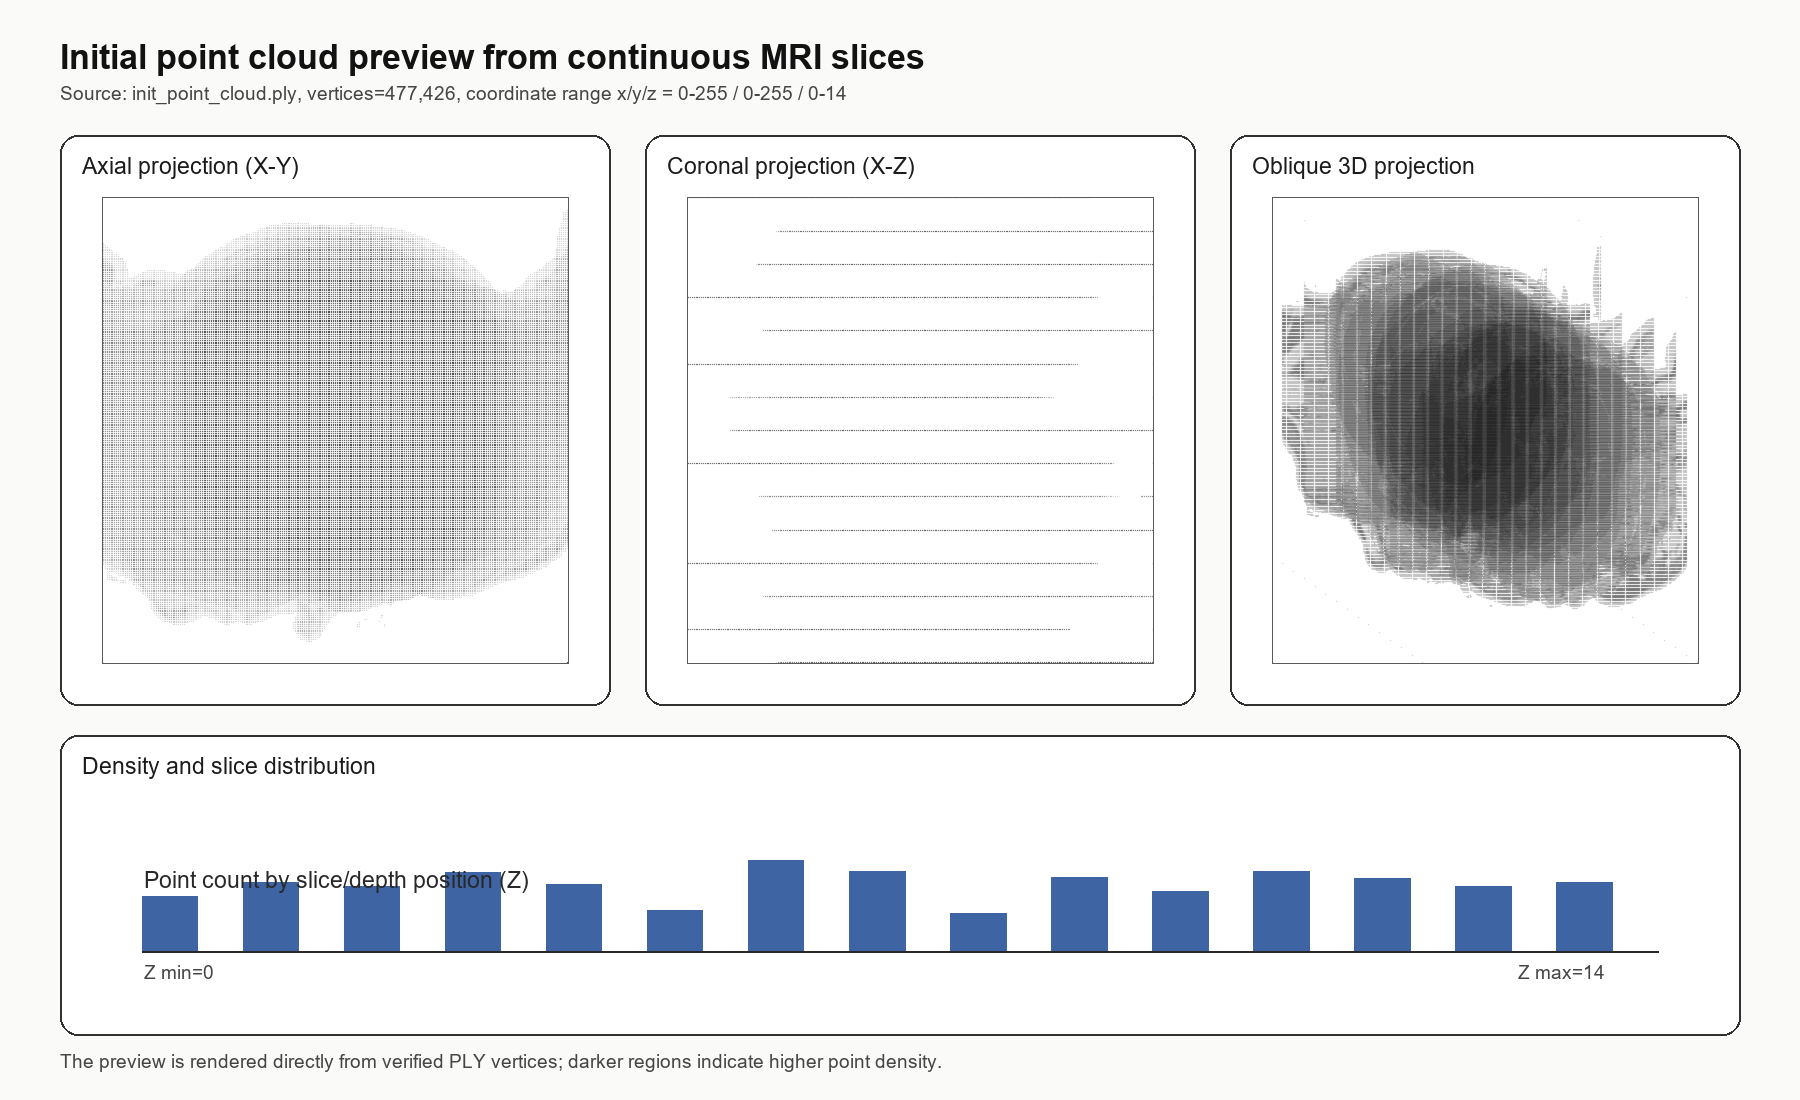
\includegraphics[width=0.82\textwidth]{figures/init_point_cloud_preview.png}
\caption{由连续 MRI 切片初始化得到的点云投影与密度分布预览}
\label{fig:init-point-cloud}
\end{figure}

该点云体现了二维切片进入三维空间的过程。每张切片对应一个 $z$ 轴位置，非背景像素对应空间点，像素灰度对应颜色强度。由此得到的点云既能作为 3DGS 三维重建输入，也能作为平台 2D/3D 对比展示的中间结果。与只展示单张二维图相比，该步骤提供了更明确的三维工程接口。

\section{3DGS 训练配置与重建结果}
3DGS 实验使用 180 张连续 MRI 切片作为监督图像，并以 300000 个点构建初始 PLY 点云。训练结果保存在 3DGS 主训练目录中。训练配置文件显示，模型采用三阶球谐函数表示颜色，输入图像目录为 \texttt{images}，数据设备为 CUDA。训练输出目录保存相机参数、checkpoint、训练日志、渲染结果和点云文件。

\begin{table}[H]
\centering
\caption{3DGS 训练主要参数与输出}
\begin{tabular}{>{\raggedright\arraybackslash}p{4.1cm}>{\raggedright\arraybackslash}p{8.2cm}}
\toprule
参数项 & 参数值或结果 \\
\midrule
训练切片数量 & 180 张 \\
训练图像分辨率 & $256\times256$ \\
初始点云规模 & 300000 点 \\
相机参数数量 & 180 个相机条目 \\
颜色表示 & 三阶球谐函数，\texttt{sh\_degree=3} \\
训练迭代次数 & 30000 轮 \\
最终 checkpoint & \texttt{chkpnt30000.pth} \\
最终点云 & 第 30000 轮输出 PLY 点云 \\
最终高斯点数量 & 572073 个 \\
\bottomrule
\end{tabular}
\end{table}

训练过程中，系统在第 1000、3000、5000、7000、15000 和 30000 轮记录训练集重建指标，也保存对应高斯点云。表 \ref{tab:3dgs-metrics} 给出了训练日志中的主要指标。随着迭代推进，L1 误差整体下降，PSNR 整体提高，说明三维高斯参数在切片监督下逐步逼近目标 MRI 切片分布。

\begin{table}[H]
\centering
\caption{3DGS 训练过程指标}
\label{tab:3dgs-metrics}
\begin{tabular}{cccc}
\toprule
迭代轮数 & L1 误差 & PSNR/dB & 说明 \\
\midrule
1000 & 0.1083 & 14.5942 & 初始优化阶段 \\
3000 & 0.0913 & 15.7418 & 结构逐步收敛 \\
5000 & 0.0881 & 15.8296 & 灰度细节增强 \\
7000 & 0.0873 & 15.8978 & 中期稳定优化 \\
15000 & 0.0806 & 16.4241 & 重建质量继续提升 \\
30000 & 0.0709 & 17.5894 & 最终训练结果 \\
\bottomrule
\end{tabular}
\end{table}

根据 180 对第 30000 轮渲染切片与参考切片计算，平均 PSNR 为 17.4738 dB，平均归一化 L1 为 0.0695，平均全局 SSIM 为 0.8935。这里的 SSIM 采用整幅灰度图全局统计方式计算，用于反映本平台实验中的重建一致性，而不是医学诊断性能指标。训练指标变化如图 \ref{fig:3dgs-metrics-30000} 所示。

\begin{figure}[H]
\centering
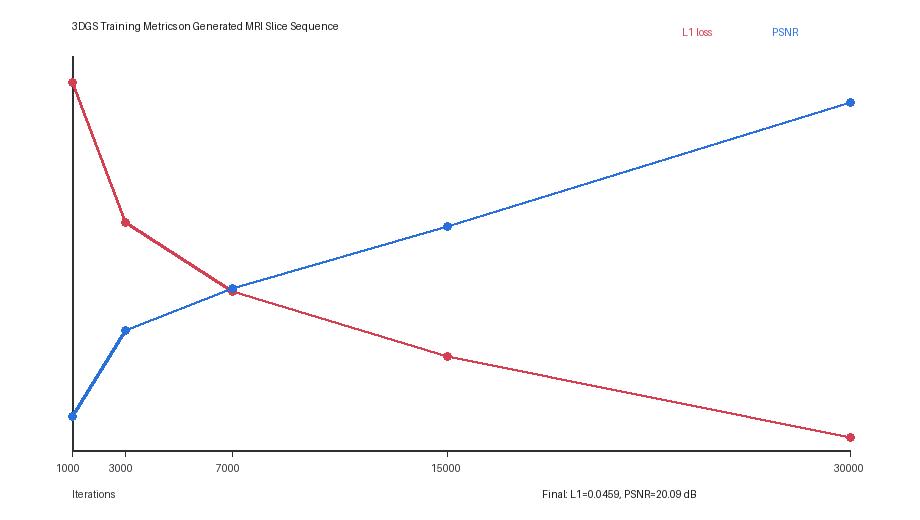
\includegraphics[width=0.9\textwidth]{figures/3dgs_metrics_30000.png}
\caption{3DGS 训练过程 L1 与 PSNR 指标变化}
\label{fig:3dgs-metrics-30000}
\end{figure}

第 30000 轮渲染切片与参考切片对比如图 \ref{fig:3dgs-comparison-30000} 所示。图中选取序列前部、中部和后部切片进行展示。渲染结果在脑部轮廓、主体灰度区域和层间变化趋势上与参考切片保持一致，但局部细节仍有一定平滑化现象。这与 MRI 灰度纹理、单序列输入约束和当前训练规模有关。

\begin{figure}[H]
\centering
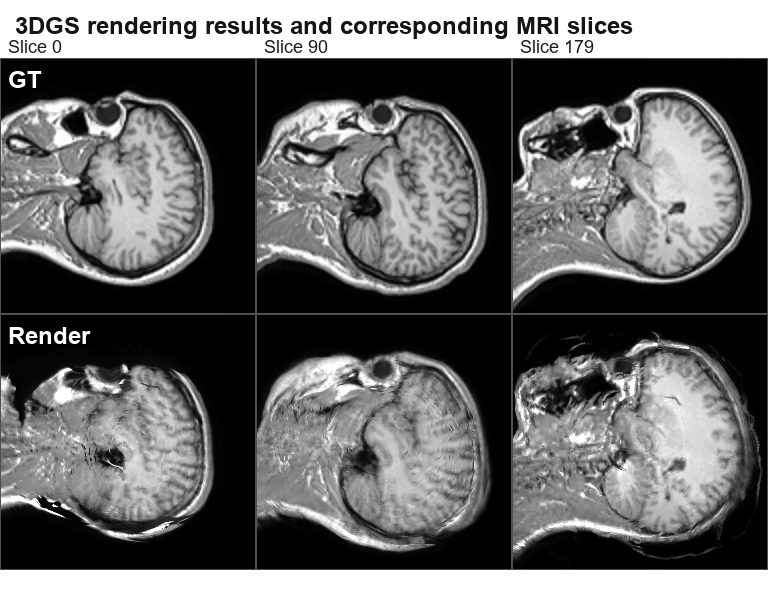
\includegraphics[width=0.82\textwidth]{figures/3dgs_slice_comparison_30000.png}
\caption{3DGS 第 30000 轮渲染切片与参考切片对比}
\label{fig:3dgs-comparison-30000}
\end{figure}

结合训练日志、checkpoint、点云文件和渲染结果可以确认，3DGS 模块已经完成训练闭环。该闭环从规则切片序列开始，并输出三维高斯表达。输入点云从 300000 点优化为 572073 个高斯点，说明训练过程在初始空间结构基础上调整并扩展了三维表达。该结果能够支撑平台开展 MRI 图像三维重建展示。

\section{综合评价与局限性分析}
本系统已经完成 MRI 数据预处理、StyleGAN2 二维生成、连续切片组织、点云初始化和 3DGS 三维重建的主要流程。StyleGAN2 部分形成了可加载权重和生成切片。3DGS 部分形成了训练日志、checkpoint、渲染图像和训练后点云。平台部分采用 FastAPI + React 架构，完成了后端接口、前端页面、任务状态、影像查看和三维展示。综合这些结果，系统满足毕业设计对算法实现、工程集成、实验验证和可视化展示的要求。

系统仍有提升空间。StyleGAN2 生成结果目前主要通过可视化和工程链路验证，后面可加入更大规模生成样本统计、专家评价或下游任务评价。3DGS 训练基于规则切片相机和单序列灰度图像，能够形成稳定的三维表达，但对细粒度组织边界的表达仍可继续改进。平台当前主要以本地 FastAPI 服务和 Vite 前端运行，后面可通过统一配置、环境变量和容器化方式提升跨环境部署能力。
